\subsection{Diferenças sobre linguagens convencionais}
\label{diferencasdsl}

Segundo \citeonline{dslengineering}, o propósito das \gls{DSL}s é de atender a um domínio específico, elas são construídas para resolver uma classe específica de problemas. De outro lado, as \gls{GPL}s são voltadas aos desenvolvedores para resolver qualquer tipo de problema computável:

\begin{citacao}
As Linguagens de Programação de Uso Geral (GPLs) são um meio para programadores instruírem computadores.Todas podem ser usadas para implementar qualquer coisa computável com uma máquina de Turing. Isso também significa que qualquer coisa expressável com uma linguagem de programação completa de Turing também pode ser expressa em qualquer outra linguagem de programação completa de Turing. Nesse sentido, todas as linguagens de programação são intercambiáveis. \cite[p.27, tradução nossa]{dslengineering}
\end{citacao}

Para \citeonline{ghosh2011dsl}, projetar uma \gls{DSL} não é uma tarefa tão assustadora quanto projetar uma linguagem de programação de uso geral. Pois tem foco limitado e é restrita apenas ao domínio que está sendo modelado.

Enquanto \gls{GPL}s são flexíveis, as \gls{DSL}s sacrificam a flexibilidade em benefício da produtividade e da concisão de programas relevantes em um domínio específico. As \gls{GPL}s são utilizadas em domínios maiores e complexos, do outro lado são trabalhados problemas menores e bem definidos \cite{dslengineering}. Algumas dessas diferenças podem ser observadas na  Figura \ref{fig:gplvsdsl}.

\begin{figure}[h!]
\centering

\caption{\textmd{DSL vs GPL}}
\label{fig:gplvsdsl}
\fcolorbox{gray}{white}{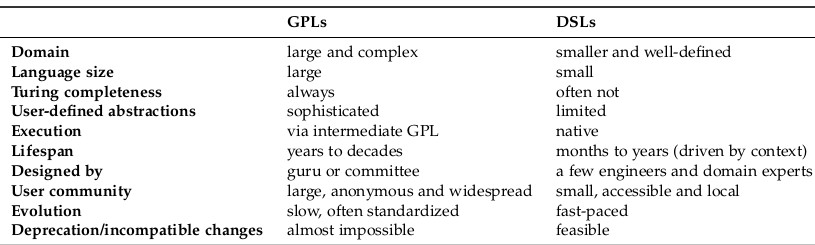
\includegraphics[width=\textwidth]{chapters/fundamentacao/imagens/gplvsdsl.jpg}}

\par\medskip\textbf{Fonte:} \citeonline{dslengineering}. \par\medskip
\end{figure}


Existem situações em que, usuários sem habilidades de programação, precisam injetar regras no sistema, ou definir condições de modo que possam atender uma funcionalidade ou requisito necessário, porém, não é viável ensiná-los conceitos básicos de linguagens de programação. A configuração usando uma linguagem específica de domínio pode ser uma alternativa para resolver estas situações \cite{novak2010easy}.  

No entanto, como em qualquer desenvolvimento de modelagem de software existem benefícios e desafios a serem levados em conta para a tomada de decisão sobre adoção \gls{DSL}s no desenvolvimento de software. Na Subseção \ref{beneficiosdsl}, são pontuados alguns desses desafios e vantagens encontrados na literatura.

\subsection{Vantagens e desafios no desenvolvimento}
\label{beneficiosdsl}

Para \citeonline{dslengineering}, o uso de \gls{DSL}s no desenvolvimento de soluções traz muitos benefícios, tais como:

\begin{enumerate}
    \item[a)] Produtividade: no sentido de que pode-se substituir muito código fonte de \gls{GPL}s, por algumas poucas linhas de código em \gls{DSL}s;
    
    \item[b)] Qualidade: quando se pensa na criação de um produto com menos \textit{bugs}, resultado da redução do grau de liberdade (desnecessário) para os programadores, prevenindo a duplicação de código (se a \gls{DSL} for projetada da maneira correta);
    
    \item[c)] Validação e Verificação: pois as \gls{DSL}s capturam suas respectivas preocupações de modo que não possuam tantos detalhes de implementação, os programas criados são semanticamente mais ricos que as \gls{GPL}s, permitindo análises e a elaboração de mensagens de erro mais significativas sobre os conceitos do domínio;
    
    \item[d)] Ferramenta de pensamento e comunicação: quando se tem uma maneira de expressar preocupações de domínio, em um idioma que está alinhado com o domínio, o pensamento se torna mais claro, porque o código que você escreve não está cheio de detalhes de implementação. Isso pode estreitar as diferenças de entendimento do domínio, que ocorrem em equipes com várias pessoas trabalhando na solução de um problema em comum;
    
    \item[e)] Envolvimento de especialistas de domínio: quando os especialistas de negócio (não desenvolvedores) conseguem expressar mais facilmente suas ideias, o que pode levar a uma melhor integração entre eles e os desenvolvedores das linguagens;
    
    \item[f)] Ferramentas produtivas: ao contrário de bibliotecas, \textit{frameworks} e \gls{DSL}s internas, as \gls{DSL}s externas podem ser fornecidas com uma \gls{IDE} preparada para o seu idioma, o que pode resultar em uma experiência de usuário muito aprimorada;

    \item[g)] Redução no \textit{Overhead}: se tratando de \gls{DSL} de geração de código, o gerador pode reduzir abstrações de domínio mais complexas e gerar código mais eficiente, assim como os compiladores das linguagens convencionais otimizam o \textit{bytecode} gerado.
\end{enumerate}

\citeonline{mernik2005and}, \citeonline{ghosh2011dsl} e \citeonline{dslengineering} apresentam em seus textos, alguns desafios e desvantagens que precisam ser consideradas antes da elaboração de uma \gls{DSL}:

\begin{enumerate}
    \item[a)] A modelagem de \gls{DSL} não é trivial, no sentido que exige muita experiência do domínio e expertise em desenvolvimento de linguagens, poucas pessoas possuem ambos;
    \item[b)] Dependendo do tamanho da comunidade de usuários da \gls{DSL}, o desenvolvimento de treinamentos, documentações, suporte e manutenção, pode se tornar um sério problema;
    \item[c)] O custo inicial de desenvolvimento pode ser alto, apesar de poder ser compensado pelo tempo economizado com o aumento da produtividade nos estágios posteriores do ciclo de desenvolvimento;
    \item[d)] A criação descontrolada de linguagens pode resultar em um design inchado, \citeonline{dslengineering} apresenta o termo \textit{DSL Hell}, no qual ao invés de pesquisar por uma \gls{DSL} existente para determinado domínio e aprendê-la, o desenvolvedor acaba por fazer a construção de uma nova linguagem, que pode possivelmente sobrepor implementações já cobertas, mas ainda assim serem incompatíveis entre si;
    \item[e)] A construção de \gls{DSL}s requer mudança no pensamento cultural da organização, pois o método de desenvolvimento é bastante diferente dos métodos tradicionais da engenharia de software, e podem implicar em mudanças significantes em como a equipe de desenvolvedores e usuários trabalham.
    
\end{enumerate}

No sentido de facilitar o design e a criação das linguagens específicas de domínio, atualmente são encontradas várias \gls{IDE}s, algumas delas são listadas na Subseção \ref{ferramentasdsl}. Elas têm como objetivo, agregar produtividade para os designers e desenvolvedores, assim como outras vantagens, compensando assim, os eventuais desafios descritos.



